% Single-column print-size preview of the target-motion figure (CVPR two-column layout).
\documentclass[10pt,twocolumn,letterpaper]{article}
\usepackage[pagenumbers]{cvpr}
\usepackage{graphicx,amsmath,lipsum}
\newsavebox{\figbox}
\begin{document}
\lipsum[1-2]
\begin{figure}[t]
\centering
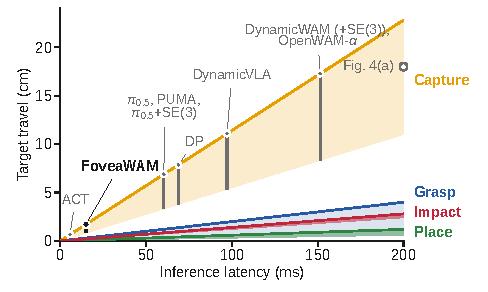
\includegraphics[width=\linewidth]{target_motion.pdf}
\caption{\textbf{Target motion during inference.} Distance $vL$ that a target travels in an inference latency $L$, over the linear speed range of each task family (Table~S1). Marks span the Capture band at each method's p95 time-to-action (Table~1); OpenWAM-$\alpha$ (off), at 466\,ms, lies off the axis. Since chunks are handed over at the next 50\,ms boundary, $vL$ is a lower bound.}
\label{fig:target_motion}
\end{figure}
\lipsum[3-8]
\end{document}
